\chapter{Basic Arithmetic and Functions}
\label{chap:ch1}
In the study of mathematics, a solid understanding of basic arithmetic operations and the concept of functions forms the foundation for more advanced topics. Arithmetic involves the manipulation of numbers through fundamental operations such as addition, subtraction, multiplication, and division. These operations are not only essential in everyday calculations but also serve as the building blocks for more complex mathematical procedures.

Functions, on the other hand, represent a crucial concept in mathematics, serving as a bridge between arithmetic and higher-level mathematical analysis. A function can be thought of as a special relationship between two sets, where each input (from the domain) is associated with exactly one output (from the co-domain). Understanding functions and their properties allows us to model and solve real-world problems with greater precision and flexibility.

In this section, we will explore the basic arithmetic rules and introduce the concept of functions, including their definitions, notations, and key properties. We will also discuss how these concepts are applied in various contexts, setting the stage for more advanced mathematical discussions.

\section{Factorisation and the Order of Operations}
Recall that when computing a product such as

\[
a(b + c) = ab + ac
\]
we distribute the factor \(a\) across each term inside the parentheses. We call this \textbf{the distributive property}. However, it is often advantageous or necessary to perform the reverse operation, known as factorisation. Factorisation involves expressing the sum \(ab + ac\) in its factored form \(a(b + c)\).

Mathematically, the expression \(a(b + c)\) is considered more simplified or "better" than \(ab + ac\). To understand why, we must distinguish between \textbf{terms} and \textbf{factors}. Terms are separated by addition or subtraction, while factors are separated by multiplication or division. For instance, the expression 

\[ 
8 - 5 + 3 
\]
consists of three terms (8, -5, and 3), whereas the expression 

\[ 
2 \times 5 \times 3 
\]
consists of three factors (2, 5, and 3). Consider the expression 

\[ 
5 + 2 + 7 \times 8 
\]
which consists of three terms (5, 2, and \(7 \times 8\)), and note that one of the terms itself contains two factors (7 and 8). Similarly, the expression 

\[ 
5(2 + 4)(-9) 
\]
consists of three factors (5, \(2 + 4\), and -9), with one factor, \(2 + 4\), containing two terms.

The advantage of expressing mathematical expressions solely in terms of factors lies in the ability to simplify them more effectively. This concept will be elaborated throughout this chapter, especially when dealing with fractions and equations. Consider the following examples of factorisation:

\[ 
8 - 5 + 3 
\]
consists of three terms (8, -5 and 3), while the expression 

\[ 
2 \times 5 \times 3 
\]
consists of three factors (2, 5 and 3). The expression 

\[ 
5 + 2 + 7 \times 8 
\]
consists of three terms (5, 2 and 7 \(\times\) 8) and one of the terms consists of two factors (7 \(\times\) 8), while the expression 

\[ 
5(2 + 4)(-9) 
\]
consists of three factors (5, (2 + 4), (-9)) and one of the factors consists of two terms ((2 + 4)).

It can be advantageous to express terms solely in factors because this allows us to simplify the expressions. This will become clearer as we progress through the lesson, and it is particularly important when working with fractions and equations. Here are some more examples of factorisation:

\begin{example} Factorisation

\begin{align*}
ab - ac &= a(b - c) \\
-ab - ac &= a(-b - c) \\
-ab - ac &= -a(b + c) \\
ab - ac + aa - aa &= a(b - c + a - a) \\
abc - ab + aba &= ab(c - 1 + a) \\
ab - abc - a &= a(b - bc - 1) = b(1 - c) - 1
\end{align*}

\end{example}

When evaluating mathematical expressions, it is crucial to follow a specific order of operations to ensure accurate results. The correct sequence for performing these operations is as follows:

\begin{enumerate}
    \item \textbf{Brackets (Parentheses)}: First, perform all operations inside brackets or parentheses.
    \item \textbf{Exponents and Radicals}: Next, evaluate exponents (powers) and radicals (roots).
    \item \textbf{Multiplication and Division}: Then, perform multiplication and division from left to right as they appear.
    \item \textbf{Addition and Subtraction}: Finally, execute addition and subtraction from left to right as they appear.
\end{enumerate}

Let's consider examples for each operation to illustrate the order of operations:

\begin{example} Brackets \newline
Evaluate the expression: \((2 + 3) \times 4\)

\[
(2 + 3) \times 4 = 5 \times 4 = 20
\]
\end{example}

\begin{example} Exponents and Radicals \newline
Evaluate the expression: \(3^2 + \sqrt{16}\)

\[
3^2 + \sqrt{16} = 9 + 4 = 13
\]
\end{example}

\begin{example} Multiplication and Division \newline
Evaluate the expression: \(6 \div 2 \times 3\). According to the standard order of operations, we perform division and multiplication from left to right:

\[
6 \div 2 \times 3 = (6 \div 2) \times 3 = 3 \times 3 = 9
\]

\end{example}

\begin{example} Addition and Subtraction \newline
Evaluate the expression: \(8 - 3 + 2\)

\[
8 - 3 + 2 = 5 + 2 = 7
\]
\end{example}

\section{Fractions}
By definition, a fraction always consists of (at least) two factors. The first factor we will call the \textbf{numerator} and is the “top part” of the fraction. The bottom part we will call the \textbf{denominator}. Perhaps the most important rule when working with fractions is that two fractions can only be added or subtracted if they have identical denominators. Also, the denominator must never be equal to 0.

\begin{example}

\[
\frac{1}{x^2 - 2}
\]    
\end{example}

Here we must make sure that \(x^2 - 2 \neq 0\) which means that we may only use values different from \(\pm\sqrt{2}\).
\begin{custombox}{Rules for Calculations Involving Fractions}
    \begin{align*}
        (1) & \quad \frac{a}{b} \times m = \frac{am}{b} \quad &\text{where } b \neq 0 \\
        (2) & \quad \frac{a}{b} \div m = \frac{a}{bm} \quad &\text{where } b \neq 0 \text{ and } m \neq 0 \\
        (3) & \quad m \div \frac{a}{b} = m \times \frac{b}{a} = \frac{mb}{a} \quad &\text{where } b \neq 0 \text{ and } a \neq 0 \\
        (4) & \quad \frac{a}{b} \times \frac{c}{a} = \frac{ac}{ba} \quad &\text{where } b \neq 0 \text{ and } a \neq 0 \\
        (5) & \quad \frac{a}{b} \div \frac{c}{a} = \frac{a}{b} \times \frac{a}{c} \quad &\text{where } b \neq 0 \text{ and } a \neq 0 \\
        (6) & \quad \frac{a}{b} = \frac{ac}{bc} \quad &\text{where } b \neq 0 \text{ and } c \neq 0 \\
        (7) & \quad \frac{a}{b} + \frac{c}{a} = \frac{aa}{ba} + \frac{cb}{ba} = \frac{aa + cb}{ba} \quad &\text{where } b \neq 0 \text{ and } a \neq 0
    \end{align*}
\end{custombox}

To extend or reduce a fraction, we must multiply or divide by the same numbers in the denominator and numerator:

\begin{example} Extending or reducing fractions

\[
\frac{72}{144} = \frac{72 \div 12}{144 \div 12} = \frac{6}{12} = \frac{6 \div 6}{12 \div 6} = \frac{1}{2}
\]

\[
\frac{2}{3} = \frac{2 \times 6}{3 \times 6} = \frac{12}{18}
\]

\[
\frac{2x}{2xx} = \frac{2}{2x}
\]

\[
\frac{3a}{6a + 3b} = \frac{3a}{3(2a + b)} = \frac{a}{2a + b}
\]    
\end{example}

To factorise an expression, all terms must be divided or multiplied uniformly. This implies that it is not possible to simplify the following expression any further, even though it might be tempting:

\[
\frac{a}{2a + b} \neq \frac{1}{2 + b}
\]

For proper factorisation of \(\frac{a}{2a + b}\), you must divide \(a\) into all terms in the denominator:

\[
\frac{a}{2a + b} = \frac{1}{2 + \frac{b}{a}}
\]

As illustrated above, the multiplication of fractions is straightforward: you multiply the numerators and denominators with each other, respectively.

\begin{example} Multiplication of fractions \newline
Consider the fractions \(\frac{a}{b}\) and \(\frac{c}{d}\). Their product is:

\[
\frac{a}{b} \times \frac{c}{d} = \frac{a \times c}{b \times d}
\]

For instance, if \(a = 2\), \(b = 3\), \(c = 4\), and \(d = 5\), then:

\[
\frac{2}{3} \times \frac{4}{5} = \frac{2 \times 4}{3 \times 5} = \frac{8}{15}
\]
  
\end{example} 

\begin{example} Dividing fractions

\[
\frac{6}{7} \div \frac{4}{21} = \frac{6}{7} \times \frac{21}{4} = \frac{126}{28} = \frac{63}{14} = \frac{9}{2}
\]

\[
\frac{1}{2} \div 3 = \frac{1}{2} \div \frac{3}{1} = \frac{1}{2} \times \frac{1}{3} = \frac{1}{6}
\]

\[
\frac{2}{3} \div \frac{8}{9} = \frac{2}{3} \times \frac{9}{8} = \frac{18}{24} = \frac{3}{4}
\]

\[
\frac{8}{9} \div 16 = \frac{8}{9} \times \frac{1}{16} = \frac{8}{144} = \frac{4}{72} = \frac{1}{18}
\]
  
\end{example}

Adding and subtracting fractions seems to cause more problems than multiplication and division. The key is to find a common denominator between the fractions and then remember the above-mentioned rule about extending fractions.

\begin{example} Adding and subtracting fractions

 \[
\frac{1}{5} + \frac{2}{5} = \frac{1 + 2}{5} = \frac{3}{5}
\]

\[
\frac{1}{4} + \frac{2}{3} = \frac{1 \times 3}{4 \times 3} + \frac{2 \times 4}{3 \times 4} = \frac{3}{12} + \frac{8}{12} = \frac{3 + 8}{12} = \frac{11}{12}
\]

\[
\frac{7}{12} - \frac{5}{8} = \frac{7 \times 8}{12 \times 8} - \frac{5 \times 12}{8 \times 12} = \frac{56}{96} - \frac{60}{96} = \frac{56 - 60}{96} = \frac{-4}{96} = \frac{-1}{24}
\]

\end{example}

Note: Never do

\[
\frac{a}{b} + \frac{c}{d} = \frac{a + b}{b + d}
\]   

\begin{example}

\[
\frac{x}{x - 1} \times \frac{2}{x(x + 4)} = \frac{2x}{(x - 1)x(x + 4)} = \frac{2}{(x - 1)(x + 4)}
\]

\[
\frac{2}{x - 1} \div \frac{x}{x - 1} = \frac{2}{x - 1} \times \frac{x - 1}{x} = \frac{2(x - 1)}{(x - 1)x} = \frac{2}{x}
\]

\[
\frac{x + 1}{x^2 + 2} + \frac{x - 6}{x^2 + 2} = \frac{x + 1 + x - 6}{x^2 + 2} = \frac{2x - 5}{x^2 + 2}
\]    
\end{example}

Remember, when a fraction is preceded by a minus sign, all signs in the numerator must be changed accordingly. This is similar to how you would change all signs within parentheses when they are preceded by a minus sign.

Consider the expression:

\[
-\frac{a - b}{c}
\]

To correctly handle the negative sign, change all the signs in the numerator:

\[
-\frac{a - b}{c} = \frac{-a + b}{c}
\]

For example, if \(a = 5\) and \(b = 3\), then:

\[
-\frac{5 - 3}{c} = \frac{-5 + 3}{c} = \frac{-2}{c}
\]

\begin{example}

\[
\frac{x + 1}{x^2 + 2} - \frac{x - 6}{x^2 + 2} = \frac{x + 1 - x + 6}{x^2 + 2} = \frac{7}{x^2 + 2}
\]    
\end{example}

\section{Exponents, Radicals and Surds}
An \textbf{exponent} is a shortcut for repeated multiplication of the same number:

\begin{example} Exponentiation

\[
4 \times 4 \times 4 \times 4 \times 4 = 4^5
\]

\[
x \times x \times x \times x \times x = x^5
\]  
\end{example}

\textbf{Radicals}, or \textbf{roots}, represent the inverse operation of applying exponents. A radical is any number expressed with the radical symbol \(\sqrt{}\). Specifically, applying a radical can reverse the effect of an exponent, and vice versa. For instance, squaring 2 yields 4, and taking the square root of 4 returns 2. Similarly, squaring 3 results in 9, and the square root of 9 brings us back to 3.

\begin{example} Taking the root

\[
\sqrt{a} \times \sqrt{a} = (\sqrt{a})^2 = a
\]

\[
\sqrt{a} = b \implies (\sqrt{a})^2 = b^2 \iff a = b^2
\]    
\end{example}



A \textbf{surd} is a type of radical that is both real and irrational, examples include \(\sqrt{2}, \sqrt{3}, \sqrt{5},\) and \(\sqrt{6}\).

Numbers can be raised to powers other than 2, such as cubing (raising to the third power), or even raising to the fourth power, the 100th power, and so forth. Correspondingly, you can take the cube root of a number, the fourth root, the 100th root, and so on. To indicate a root other than a square root, the same radical symbol is used, but with a number called the index inserted into the radical sign, typically positioned within the "check mark" part.

\begin{example} Index and argument

\[
4^3 = 64 \iff \sqrt[3]{64} = 4
\]
   
\end{example}

In this example, the "3" inside the radical sign is the \textbf{index} of the radical. The "64" is referred to as the argument of the \textbf{radical}, also known as the \textbf{radicand}. Since square roots are the most common type of radicals, the index is usually omitted for square roots. Although "\(\sqrt[2]{2}\)" would be technically correct, it is rarely used in practice.
\begin{custombox}{Rules for calculations involving radicals}
    \begin{align*}
    &(1) \quad \sqrt[n]{x y}=\sqrt[n]{x} \times \sqrt[n]{y}   &   &\textnormal{where } x,y \geq 0\\
    &(2) \quad \sqrt[n]{\frac{x}{y}} = \frac{\sqrt[n]{x}}{\sqrt[n]{y}}    &   &\textnormal{where } x \geq 0 \textnormal{ and } y > 0 \\
    &(3) \quad \sqrt{x^2} = |x|   &   &\textnormal{where } x \in \mathbb{R} \\
    &(4) \quad (\sqrt[n]{x})^n = x    &   &\textnormal{If } x < 0 \textnormal{ and } n \in \mathbb{N}, \textnormal{then } \sqrt[n]{x} \textnormal{ is not defined}\\
    &(5) \quad \sqrt[n]{-x}=-\sqrt[n]{x}  &   &\textnormal{where } x \geq 0 \textnormal{ and } n \in \mathbb{N} \textnormal{ is odd }
    \end{align*}
\end{custombox}

Raising a number to a \textbf{power}, also known as \textbf{exponentiation}, is a fundamental mathematical operation that involves multiplying a number by itself a certain number of times as we saw above. The \textbf{base} is the number being multiplied, and the \textbf{exponent} indicates how many times the base is used as a factor. For example, \(a^n\) means that the base \(a\) is multiplied by itself \(n\) times. Exponentiation is a powerful tool in mathematics, with a few essential rules that govern its application.
\begin{custombox}{Rules for calculations involving exponents 1}
\label{def:DefPow}
$\textnormal{Let } n,m \in \mathbb{N}\textnormal{. Then the following applies:}$
\begin{fleqn}
\begin{alignat*}{2}
&(1) \hspace{1cm} x^n \cdot x^m=x^{n+m}  \\
&(2) \hspace{1cm} \frac{x^n}{x^m}=x^{n-m}   &\qquad&   x \neq 0  \\
&(3) \hspace{1cm} x^n \cdot y^n=(x \cdot y)^n \\
&(4) \hspace{1cm} \frac{x^n}{y^n}=\left(\frac{x}{y}\right)^n &\qquad& y \neq 0 \\
&(5) \hspace{1cm} \left(x^n\right)^m=x^{n \cdot m}\\
&(6) \hspace{1cm} x^1=x
\end{alignat*}
\end{fleqn}
\end{custombox}

Some of these rules allow the concept of powers to be extended so that the exponent may be any integer. If you set \(n = m\) in rule (2), you get:

\[
\frac{x^n}{x^n} = x^{n-n} = x^0
\]

But since \(\dfrac{x^n}{x^n} = 1\), we obtain

\[
x^0 = 1
\]

Thus, the concept of exponentiation is extended to include \(n \in \mathbb{N} \cup \{0\}\). If you now set \(n = 0\) again in rule (2), you get:

\[
\frac{x^0}{x^m} = x^{0-m} = x^{-m}
\]

But according to the previous calculation, \(x^0 = 1\). Therefore, you obtain

\begin{equation*}
 \frac{1}{x^m} = x^{-m}   
\end{equation*}

Since \(m\) is a positive number, \(-m\) must be a negative number. Thus, the concept of exponentiation is extended to apply to all integers. This means that definition our concept of powers holds for \(n \in \mathbb{Z}\) and that the rules in definition \ref{def:DefPow} apply for \(n \in \mathbb{Z}\) and \(m \in \mathbb{Z}\). As a consequence, the following rules can be added:
\begin{custombox}{Rules for calculations involving exponents 2}
$\textnormal{Let } n \in \mathbb{Z} \textnormal{. Then the following applies:}$
\begin{fleqn}
\begin{alignat*}{2}
&(7) \hspace{1cm} x^0=1   &\qquad&   x \neq 0  \\
&(8) \hspace{1cm} \frac{1}{x^m}=x^{-m} &\qquad& x \neq 0 \\
\end{alignat*}
\end{fleqn}
\end{custombox}

Let us illustrate these rules with a couple of examples.

\begin{example} Reduce the following expression

    \begin{equation*}
\left(3 x y^6\right)^3=3^3 \cdot x^3 \cdot\left(y^6\right)^3=27 x^3 y^{18}
\end{equation*}
\end{example}

\begin{example} Reduce the following expression

\begin{equation*}
\frac{a^{-4} b^3}{a^7 b^{-5}}=\frac{a^{-4}}{a^7} \cdot \frac{b^3}{b^{-5}}=a^{-4-7} \cdot b^{3-(-5)}=a^{-11} \cdot b^8=\frac{b^8}{a^{11}}
\end{equation*}
\end{example}

For positive numbers \(x\), the concept of exponentiation can be further extended to apply when the exponent is a rational number. Any rational number \(r \in \mathbb{Q}\) can be written as \(r = \dfrac{m}{n}\), where \(m \in \mathbb{Z}\) and \(n \in \mathbb{N}\). For \(x > 0\), we now define

\begin{equation*}
y=x^r=x^{\frac{m}{n}}
\end{equation*}

From this, you obtain (using, among other things, rule (5)):

\[
y^n = \left(x^{\frac{m}{n}}\right)^n = x^{\frac{m}{n} \cdot n} = x^m
\]

Finally, by using the concept of radicals, we obtain

\begin{equation*}
 y^n=x^m \quad \iff \quad y=\sqrt[n]{x^m}   
\end{equation*}

Note that because \(x > 0\), it follows that \(y > 0\) as well. We are now ready to state \textbf{\textit{the extended concept of exponentiation}}.

\begin{custombox}{The extended concept of exponentiation}
$\textnormal{Let } m \in \mathbb{Z} \textnormal{ and let }  n \in \mathbb{N} \textnormal{ such that } \dfrac{m}{n} \in \mathbb{Q}  \textnormal{. Then the following applies:}$

\[
x^{\frac{m}{n}} = \sqrt[n]{x^m} \hspace{1cm} x > 0
\]

\textnormal{And more specifically, the following holds true}

\[
x^{\frac{1}{n}} = \sqrt[n]{x} \hspace{1.3cm} x > 0
\]

\end{custombox}

The denominator of a rational exponent corresponds to the index of the radical, while the numerator remains as the exponent of the base. Conversely, the index of a radical can be transformed into the denominator of an exponent in an equivalent exponential expression. This property allows us to convert any radical expression into an exponential form, providing a powerful tool for simplification.

\begin{example}

\[
\sqrt[5]{x^3} = x^{\frac{3}{5}} \quad  \textnormal{vs.} \quad \sqrt[3]{x^5} = x^{\frac{5}{3}}
\]

\[
\frac{1}{\sqrt[7]{x^3}} = x^{-\frac{3}{7}}
\]

\[
\frac{1}{\sqrt[3]{x^2}} = \left(x^2\right)^{-\frac{2}{3}}
\]
\end{example}

This property can also be reversed: any rational exponent can be rewritten as a radical expression by using the denominator as the radical's index. The ability to interchange between exponential and radical forms enables us to evaluate expressions that were previously difficult to handle by converting them into radicals.

\begin{example}
\[
27^{-\frac{4}{3}} = \frac{1}{\sqrt[3]{27^4}} = \frac{1}{\left(\sqrt[3]{27}\right)^4} = \frac{1}{3^4} = \frac{1}{81}
\]    
\end{example}

One of the greatest advantages of converting a radical expression into an exponential form is that it allows us to apply all the properties of exponents to simplify the expression. The following examples illustrate how various properties can be utilised to simplify expressions with rational exponents.

\begin{example}

\[
a^{\frac{2}{3}}b^{\frac{1}{2}}a^{\frac{1}{6}}b^{\frac{1}{5}} = a^{\frac{2}{3}+\frac{1}{6}}b^{\frac{1}{2}+\frac{1}{5}} = a^{\frac{4}{6}+\frac{1}{6}}b^{\frac{5}{10}+\frac{2}{10}} = a^{\frac{5}{6}}b^{\frac{7}{10}}
\]

\[
\left( x^{\frac{1}{3}} x^{\frac{2}{5}} \right)^{\frac{3}{4}} = x^{\frac{1}{3} \times \frac{3}{4}} x^{\frac{2}{5} \times \frac{3}{4}} = x^{\frac{3}{12}} x^{\frac{6}{20}} = x^{\frac{1}{4}} x^{\frac{3}{10}} = x^{\frac{11}{20}}
\]

\[
\frac{x^{\frac{4}{2}}x^{\frac{4}{6}}x^{\frac{1}{2}}x^{\frac{5}{6}}}{x^{\frac{7}{2}}x^0} = 2x^{\frac{4}{2}+\frac{1}{2}}x^{\frac{4}{6}+\frac{5}{6}} x^{\frac{7}{2}} = 2x^{\frac{5}{2}} x^{\frac{9}{6}} x^{\frac{7}{2}} = 2x^{-1} x^{\frac{3}{2}} = 2x^{\frac{1}{2}}
\]

\[
\left( 25x^{\frac{1}{3}} x^{\frac{2}{5}} \right)^{-\frac{1}{2}} = \left( 25x^{\frac{5}{15}} x^{\frac{4}{10}} \right)^{-\frac{1}{2}} = \left( 25x^{-\frac{7}{15}} x^{\frac{19}{10}} \right)^{-\frac{1}{2}} = \left( \frac{9}{25x^{-\frac{7}{15}}x^{\frac{19}{10}}} \right)^{\frac{1}{2}} = \frac{9}{2} \cdot 25x^{-\frac{7}{30}} x^{\frac{19}{20}} = \frac{3x^{\frac{7}{30}}}{5x^{\frac{19}{20}}}
\]
\end{example}

It is important to remember that when simplifying expressions with rational exponents, we are applying the same exponent rules that are used for integer exponents. The only difference is that we must also adhere to the rules for fractions.

\section{Using Formulae and Substitution}
In the study of engineering, physical quantities are often related to each other through formulas. These formulas consist of variables and constants that represent the physical quantities in question. To evaluate a formula, one must substitute numerical values for the variables.

For example, Ohm’s law provides a formula that relates the voltage, \(v\), across a resistor with a resistance value \(R\), to the current \(i\) flowing through it. The formula is given by

\[
v = iR
\]

This formula allows us to calculate the voltage \(v\) if the values for \(i\) and \(R\) are known. For instance, if \(i = 13 \, \text{A}\) and \(R = 5 \, \Omega\), then

\[
v = iR = (13)(5) = 65
\]

Thus, the voltage is 65 V.

This example highlights the importance of paying close attention to the units of any physical quantities involved. A formula is only valid if a consistent set of units is used.

\begin{example} Inserting into formulae \newline
The kinetic energy \(K\) of an object with mass \(M\) moving at speed \(v\) can be calculated using the formula:

\[
K = \frac{1}{2}Mv^2
\]

Calculate the kinetic energy of an object with a mass of 5 kg moving at a speed of \(2 \, \text{m} \, \text{s}^{-1}\).

\begin{solution}
\[
K = \frac{1}{2}Mv^2 = \frac{1}{2}(5)(2^2) = 10
\] 

\end{solution}

In the SI system, the unit of energy is the joule, so the kinetic energy of the object is 10 joules.
\end{example}

\begin{example} Inserting into formulae \newline
The area \(A\) of a circle with radius \(r\) can be calculated using the formula \(A = \pi r^2\).

Alternatively, if the diameter \(d\) of the circle is known, the equivalent formula can be used:

\[
A = \frac{\pi d^2}{4}
\]

Calculate the area of a circle with a diameter of 0.1 m. The value of \(\pi\) is pre-programmed in your calculator.

\begin{solution}
    \[
A = \frac{\pi (0.1)^2}{4} = 0.00785 \, \text{m}^2
\]

\end{solution}


\end{example}

\begin{example} Inserting into formulae \newline
The volume \(V\) of a circular cylinder is equal to its cross-sectional area \(A\) multiplied by its length \(h\).

Calculate the volume of a cylinder with a diameter of 0.1 m and a length of 0.3 m.

\begin{solution}
  \[
V = Ah = \frac{\pi (0.1)^2}{4} \times 0.3 = 0.00236
\]

The volume is \(0.00236 \, \text{m}^3\).
\end{solution}
\end{example}

\section{Rearranging Formulae}
In the formula for the area of a circle, \(A = \pi r^2\), the variable \(A\) is referred to as the subject of the formula. A variable is considered the subject if it appears by itself on one side of the equation, usually on the left-hand side, and nowhere else in the formula. If we are asked to transpose the formula for \(r\), or solve for \(r\), we must rearrange the equation so that \(r\) becomes the subject. When transposing a formula, any operation performed on one side must also be applied to the other side. There are five key rules to follow during this process.

\begin{custombox}{Rules for rearranging formulae}
The following operations can be performed on both sides of the formula:
\begin{itemize}
    \item Add the same quantity to both sides
    \item Subtract the same quantity from both sides
    \item Multiply both sides by the same quantity - remember to multiply all terms
    \item Divide both sides by the same quantity - remember to divide all terms
    \item Apply a function to both sides, such as squaring or finding the reciprocal
\end{itemize}
\end{custombox}

\begin{example} Transpose the formula \(p = 5t - 17\) to make \(t\) the subject.

\begin{solution}
 To isolate \(t\) on the left-hand side, proceed in steps using the five rules. First, add 17 to both sides of the equation \(p = 5t - 17\):
\[
p + 17 = 5t - 17 + 17
\]
Simplifying, we get:
\[
p + 17 = 5t
\]
Next, divide both sides by 5 to isolate \(t\):
\[
\frac{p + 17}{5} = t
\]
Thus, the formula for \(t\) is:
\[
t = \frac{p + 17}{5}
\]   
\end{solution}    
\end{example}

\begin{example} Transpose the formula \(\sqrt{2q} = p\) to solve for \(q\).

\begin{solution}
   First, square both sides to eliminate the square root around \(2q\). Note that \((\sqrt{2q})^2 = 2q\). This gives:
\[
2q = p^2
\]
Next, divide both sides by 2 to solve for \(q\):
\[
q = \frac{p^2}{2}
\]   
\end{solution}
 
\end{example}



\begin{problem}
Transpose the formula \(v = \sqrt{t^2 + w}\) to solve for \(w\). To isolate \(w\), follow these steps:   
\end{problem}

    \begin{enumerate}[a.]
        \item First, square both sides to eliminate the square root around \(t^2 + w\):
        \[
        v^2 = t^2 + w
        \]

        \item Next, subtract \(t^2\) from both sides to isolate \(w\):
        \[
        v^2 - t^2 = w
        \]

        \item Finally, write down the formula for \(w\):
        \[
        w = v^2 - t^2
        \]
    \end{enumerate}

\begin{example} Transpose the formula \(x = \frac{1}{y}\) to solve for \(y\).

\begin{solution}
To isolate \(y\), notice that \(y\) appears in the denominator. Multiplying both sides by \(y\) removes the fraction:

\[
yx = y \times \frac{1}{y}
\]

This simplifies to:

\[
yx = 1
\]

Finally, divide both sides by \(x\) to solve for \(y\):
\[
y = \frac{1}{x}
\]

Alternatively, you can simply invert both sides directly to obtain:

\[
y = \frac{1}{x}
\]    
\end{solution}


\end{example}


\begin{example} Make \(R\) the subject of the formula:

\[
\frac{2}{R} = \frac{3}{x + y}
\]

\begin{solution} Since \(R\) appears in a fraction, invert both sides:

\[
\frac{R}{2} = \frac{x + y}{3}
\]

Multiplying both sides by 2 yields: $R = \dfrac{2(x + y)}{3}$    
\end{solution}
    
\end{example} 

\begin{example} Make \(R\) the subject of the formula:

\[
\frac{1}{R} = \frac{1}{R_1} + \frac{1}{R_2}
\]
\begin{solution}
The two terms on the right-hand side can be combined:
\[
\frac{1}{R_1} + \frac{1}{R_2} = \frac{R_2 + R_1}{R_1R_2}
\]

The formula then becomes:
\[
\frac{1}{R} = \frac{R_2 + R_1}{R_1R_2}
\]

Finally, inverting both sides gives:
\[
R = \frac{R_1R_2}{R_2 + R_1}
\]

\end{solution}
\end{example}

\section{Functions}
In mathematics, a function assigns each element of one set to a specific element of another set (which may be the same set). For example, consider a Mathematics for Software Engineering class where each student is assigned a grade from the set \(\{12, 10, 7, 4, 02\}\). Suppose the grades are as follows:

\begin{figure}[h]
    \centering
    \begin{tikzpicture}[>=Stealth] % Stealth is a nice arrow style
        % Left column of names
        \node (A1) at (0,0) {Alice};
        \node (A2) at (0,-1) {Bob};
        \node (A3) at (0,-2) {Carol};
        \node (A4) at (0,-3) {Dave};
        \node (A5) at (0,-4) {Eve};
        
        % Right column of numbers
        \node (B1) at (4,0) {$12$};
        \node (B2) at (4,-1) {$10$};
        \node (B3) at (4,-2) {$7$};
        \node (B4) at (4,-3) {$4$};
        \node (B5) at (4,-4) {$02$};
        
        % Connecting lines with arrows
        \draw[->, thick, black] (A1.east) -- (B1.west);
        \draw[->, thick, black] (A2.east) -- (B3.west);
        \draw[->, thick, black] (A3.east) -- (B2.west);
        \draw[->, thick, black] (A4.east) -- (B1.west);
        \draw[->, thick, black] (A5.east) -- (B5.west);
    \end{tikzpicture}
    \caption{Example of a function mapping names to numbers.}
    \label{fig:names_to_numbers}
\end{figure}


This assignment of grades, illustrated in figure \ref{fig:names_to_numbers}, exemplifies a function.

Functions play a crucial role in mathematics and computer science. They define discrete structures such as sequences and strings and are used to analyse the time complexity of algorithms. Many computer programs are designed to compute values of functions. Recursive functions, defined in terms of themselves, are especially significant in computer science. This section provides an overview of the fundamental concepts of functions needed in the mathematics for software engineering.

\begin{definition}
Let $A$ and $B$ be nonempty sets. A function $f$ from $A$ to $B$ is an assignment of exactly one element of $B$ to each element of $A$. We write $f(a)=b$ if $b$ is the unique element of $B$ assigned by the function $f$ to the element $a$ of $A$. If $f$ is a function from $A$ to $B$, we write $f: A \rightarrow B$.
\end{definition}

\begin{remark}
    Functions are sometimes also called mappings or transformations.
\end{remark}

Functions can be specified in various ways. Sometimes, we explicitly state the assignments, as shown in Figure \ref{fig:names_to_numbers}. Often, a formula such as \(f(x) = x + 1\) is used to define a function. In other cases, a computer program may specify the function.

\begin{definition}
If $f$ is a function from $A$ to $B$, we say that $A$ is the \textbf{domain} of $f$ and $B$ is the \textbf{co-domain} of $f$. If $f(a)=b$, we say that $b$ is the \textbf{image} of $a$ and $a$ is a \textbf{preimage} of $b$. The \textbf{range}, or image, of $f$ is the set of all images of elements of $A$. Also, if $f$ is a function from $A$ to $B$, we say that $f$ \textbf{maps} $A$ to $B$.    
\end{definition}

When defining a function, we specify its domain, co-domain, and the mapping of elements from the domain to the co-domain. Two functions are equal if they have the same domain, the same co-domain, and map each element of their domain to the same element in the co-domain. 

It's important to note that altering the domain or co-domain results in a different function. Similarly, changing the mapping of elements also produces a different function.


\begin{figure}[h]
\centering
\begin{tikzpicture}[>=Stealth, node distance=4cm, thick, scale=1]

    % Draw larger circles for sets A and B
    \draw[thick] (0,0) circle [radius=1.5cm] node at (0, 2) {\Large $A$};
    \draw[thick] (6,0) circle [radius=1.5cm] node at (6, 2) {\Large $B$};

    % Place larger nodes for elements a and b=f(a)
    \node[fill, circle, inner sep=2pt, label=below:{$a$}] (a) at (0,0.3) {};
    \node[fill, circle, inner sep=2pt, label=below:{$b=f(a)$}] (b) at (6,0.3) {};

    % Draw the larger straight arrow representing f
    \draw[->, ultra thick, black] (a) -- (b) node[midway, above] {\Large $f$};

    % Draw the curved arrow representing f at the bottom, touching the circles
    \draw[->, ultra thick, black, bend right=30] ([shift={(270:1.5cm)}]0,0) 
    to node[midway, below] {\Large $f$} 
    ([shift={(270:1.5cm)}]6,0);

\end{tikzpicture}
\caption{A function \(f\) mapping an element \(a\) from set \(A\) to an element \(b=f(a)\) in set \(B\).}
\label{fig:function_mapping}
\end{figure}

The following examples illustrate various functions. In each example, we describe the domain, co-domain, range, and the assignment of values to the elements of the domain.

\begin{example} What are the domain, co-domain, and range of the function that assigns grades to students described in the first paragraph of the introduction of this section?

\begin{solution}
    Let $G$ be the function that assigns a grade to a student in our Software engineering mathematics class. Note that $G$(Alice) $=12$, for instance. The domain of $G$ is the set \{Alice, Bob, Carol, David, Eve $\}$, and the co-domain is the set $\{12, 10, 7, 4, 02\}$. The range of $G$ is the set $\{12, 10, 7, 02\}$, because each grade except $4$ is assigned to some student.
\end{solution}
    
\end{example}

\begin{example}
    Let $f$ be the function that assigns the last two bits of a bit string of length 2 or greater to that string. For example, $f(11010)=10$. Then, the domain of $f$ is the set of all bit strings of length 2 or greater, and both the co-domain and range are the set $\{00,01,10,11\}$.
\end{example}

\begin{example}
    Let $f: \mathbb{Z} \rightarrow \mathbb{Z}$ assign the square of an integer to this integer. Then, $f(x)=x^2$, where the domain of $f$ is the set of all integers, the co-domain of $f$ is the set of all integers, and the range of $f$ is the set of all integers that are perfect squares, namely, $\{0,1,4,9, \ldots\}$.
\end{example}

\subsection*{One-to-One and Onto Functions}
In mathematics, functions are a fundamental concept used to describe the relationship between two sets. However, not all functions behave the same way. To understand these differences, we introduce the concepts of one-to-one (injective) and onto (surjective) functions.

Some functions never assign the same value to two different domain elements. These functions are said to be \textbf{one-to-one}.

\begin{definition} {One-to-One functions (Injective)}
A function \( f: A \rightarrow B \) is called \textbf{one-to-one} (or \textbf{injective}) if different elements in \( A \) map to different elements in \( B \). In other words, if \( f(a_1) = f(a_2) \), then \( a_1 = a_2 \). This property ensures that no two distinct elements in \( A \) are mapped to the same element in \( B \).     
\end{definition}

Graphically, a function is one-to-one if no horizontal line intersects the graph of the function at more than one point.

\begin{definition}{Onto Functions (Surjective)}
A function \( f: A \rightarrow B \) is called \textbf{onto} (or \textbf{surjective}) if every element in \( B \) is the image of at least one element in \( A \). In other words, for every \( b \in B \), there exists at least one \( a \in A \) such that \( f(a) = b \). This property ensures that the function ``covers'' the entire set \( B \).
\end{definition}

\subsection*{Inverse Functions}

Now, consider a function \( f: A \rightarrow B \) that is both one-to-one and onto. Because \( f \) is onto, every element of \( B \) is the image of some element in \( A \). Furthermore, because \( f \) is one-to-one, every element of \( B \) is the image of a unique element of \( A \). This unique correspondence allows us to define a new function from \( B \) to \( A \) that ``reverses'' the mapping given by \( f \).

\begin{figure}[h]
\centering
\begin{tikzpicture}[>=Stealth, thick, scale = 1.5]

% Draw circles representing sets A and B
\draw (0,0) circle (1.5cm);
\draw (6,0) circle (1.5cm);

% Labels for sets A and B
\node at (0,-1) {A};
\node at (6,-1) {B};


% Points in sets with adjusted labels
\node[fill=black, circle, inner sep=1.5pt, label={[xshift=-0.6cm]below:{$a = f^{-1}(b)$}}] (A1) at (0,0.7) {};
\node[fill=black, circle, inner sep=1.5pt, label={[xshift=0.5cm]below:{$b = f(a)$}}] (B1) at (6,0.7) {};


% Arrows for f and f^{-1}
\draw[->] (A1) to[bend left=30] node[midway, above] {$f(a)$} (B1);
\draw[->] (B1) to[bend left=30] node[midway, below] {$f^{-1}(b)$} (A1);

% Arrows for f and f^{-1} below the main circles
\draw[->] (0.6,-1.5) to[bend left=20] node[midway, above] {$f$} (5.4,-1.5);
\draw[->] (5.4,-1.8) to[bend left=20] node[midway, below] {$f^{-1}$} (0.6,-1.8);

\end{tikzpicture}
\caption{The function $f^{-1}$ is the inverse of function $f$.}
\label{fig:inv}
\end{figure}

This new function is called the \textbf{inverse function} of \( f \), denoted by \( f^{-1}: B \rightarrow A \). The inverse function \( f^{-1} \) satisfies the following properties:

\[
f(f^{-1}(b)) = b \quad \text{for every } b \in B.
\]
\[
f^{-1}(f(a)) = a \quad \text{for every } a \in A.
\]

We can summarise these considerations in the following definition

\begin{definition}{Inverse Functions}
Let $f$ be a one-to-one correspondence from the set $A$ to the set $B$. The inverse function of $f$ is the function that assigns to an element $b$ belonging to $B$ the unique element $a$ in $A$ such that $f(a)=b$. The inverse function of $f$ is denoted by $f^{-1}$. Hence, $f^{-1}(b)=a$ when $f(a)=b$.    
\end{definition}

These properties show that \( f^{-1} \) effectively undoes the work of \( f \), mapping each element of \( B \) back to the corresponding element in \( A \).

\begin{example}


Let \( f: \mathbb{R} \rightarrow \mathbb{R} \) be defined by \( f(x) = 2x + 3 \). We can check that \( f \) is both one-to-one and onto:

\begin{itemize}
    \item \textbf{One-to-One}: If \( f(x_1) = f(x_2) \), then \( 2x_1 + 3 = 2x_2 + 3 \). Subtracting 3 from both sides gives \( 2x_1 = 2x_2 \), and dividing by 2 yields \( x_1 = x_2 \). Thus, \( f \) is one-to-one.
    \item \textbf{Onto}: Given any \( y \in \mathbb{R} \), we can solve \( y = 2x + 3 \) for \( x \) to find \( x = \frac{y - 3}{2} \). Since this \( x \) exists for every \( y \), \( f \) is onto.
\end{itemize}

Since \( f \) is both one-to-one and onto, it has an inverse function \( f^{-1} \) defined by

\[
f^{-1}(y) = \frac{y - 3}{2}.
\]

  
\end{example}

\subsection*{Composite Functions}
In mathematics, functions can be combined to form new functions. One important way of combining functions is through the composition of functions. The composite of two functions is essentially applying one function to the results of another.

\begin{figure}[h]
\centering
\begin{tikzpicture}[>=Stealth, thick]

% Draw circles representing sets A, B, and C
\draw (0,0) circle (1.5cm);  % Set A
\draw (5,0) circle (1.5cm);  % Set B
\draw (10,0) circle (1.5cm); % Set C

% Labels for sets A, B, and C
\node at (0,-1) {A};
\node at (5,-1) {B};
\node at (10,-1) {C};

% Points in sets with adjusted labels
\node[fill=black, circle, inner sep=1.5pt, label={[xshift=-0.1cm]below:{$a$}}] (A) at (0,0.7) {};

\node[fill=black, circle, inner sep=1.5pt, label=below:{$g(a)$}] (B) at (5,0.7) {};
\node[fill=black, circle, inner sep=1.5pt, label={[xshift=0.4cm]below:{$f(g(a))$}}] (C) at (10,0.7) {};

% Arrows for g and f
\draw[->] (A) to[bend left=15] node[midway, above] {$g(a)$} (B);
\draw[->] (B) to[bend left=15] node[midway, above] {$f(g(a))$} (C);
\draw[->] ([shift={(360:1.5cm)}]0,0) to node[midway, below] {$g$} (3.5,0);
\draw[->] ([shift={(360:0cm)}]6.5,0) to node[midway, below] {$f$} (8.5,0);

% Arrows for f ∘ g and (f ∘ g)(a)
\draw[->] (A) to[bend left=40] node[midway, above] {$(f \circ g)(a)$} (C);
% Draw the curved arrow representing f at the bottom, touching the circles
\draw[->, bend right=20] ([shift={(270:1.5cm)}]0,0) to node[midway, below] {$f \circ g$} ([shift={(270:1.5cm)}]10,0);

\end{tikzpicture}
\caption{The composition of $f$ and $g$.}
\label{fig:composite}
\end{figure}

\begin{definition}
    

Let \( f: B \rightarrow C \) and \( g: A \rightarrow B \) be two functions. The \textbf{composite function} of \( f \) and \( g \), denoted by \( f \circ g \), is a function from \( A \) to \( C \) defined by

\[
(f \circ g)(x) = f(g(x)),
\]

for every \( x \in A \).

\end{definition}

In other words, the composite function \( f \circ g \) means that you first apply the function \( g \) to the input \( x \), and then apply the function \( f \) to the result of \( g(x) \). In figure \ref{fig:composite} the composition of functions is shown.

\begin{example}
    

Consider the functions \( f(x) = 2x + 3 \) and \( g(x) = x^2 \). The composite function \( f \circ g \) is given by:

\[
(f \circ g)(x) = f(g(x)) = f(x^2) = 2x^2 + 3.
\]

Here, the function \( g(x) \) squares the input \( x \), and then the function \( f(x) \) multiplies the result by 2 and adds 3.
\end{example}

Now, let's reverse the composition and compute \( g \circ f \):

\[
(g \circ f)(x) = g(f(x)) = g(2x + 3) = (2x + 3)^2.
\]

Notice that \( f \circ g \) and \( g \circ f \) are generally different functions, illustrating that the composition of functions is not commutative.

\begin{example}
    Let $g$ be the function from the set $\{a, b, c\}$ to itself such that $g(a)=b, g(b)=c$, and $g(c)=a$. Let $f$ be the function from the set $\{a, b, c\}$ to the set $\{1,2,3\}$ such that $f(a)=3, f(b)=2$, and $f(c)=1$. What is the composition of $f$ and $g$, and what is the composition of $g$ and $f$ ?

    \begin{solution}
        The composition $f \circ g$ is defined by $(f \circ g)(a)=f(g(a))=f(b)=2$, $(f \circ g)(b)=f(g(b))=f(c)=1$, and $(f \circ g)(c)=f(g(c))=f(a)=3$.
        
        Note that $g \circ f$ is not defined, because the range of $f$ is not a subset of the domain of $g$.
    \end{solution}
\end{example}


\begin{example}{label:}
Let $f$ and $g$ be the functions from the set of integers to the set of integers defined by $f(x)=2 x+3$ and $g(x)=3 x+2$. What is the composition of $f$ and $g$ ? What is the composition of $g$ and $f$?

\begin{solution}
Both the compositions $f \circ g$ and $g \circ f$ are defined. Moreover,
\[
(f \circ g)(x)=f(g(x))=f(3 x+2)=2(3 x+2)+3=6 x+7
\]
and
\[
(g \circ f)(x)=g(f(x))=g(2 x+3)=3(2 x+3)+2=6 x+11 .
\]
\end{solution}
\end{example}

\begin{remark}
Even though \( f \circ g \) and \( g \circ f \) are defined for the functions \( f \) and \( g \) in example 35, \( f \circ g \) and \( g \circ f \) are not equal. In other words, the commutative law does not hold for the composition of functions.
  
\end{remark}

When the composition of a function and its inverse is formed, in either order, an identity function is obtained. To see this, suppose that \( f \) is a one-to-one correspondence from the set \( A \) to the set \( B \). Then the inverse function \( f^{-1} \) exists and is a one-to-one correspondence from \( B \) to \( A \). The inverse function reverses the correspondence of the original function, so \( f^{-1}(b)=a \) when \( f(a)=b \), and \( f(a)=b \) when \( f^{-1}(b)=a \).

Hence,

\[
\left(f^{-1} \circ f\right)(a) = f^{-1}(f(a)) = f^{-1}(b) = a,
\]

and

\[
\left(f \circ f^{-1}\right)(b) = f\left(f^{-1}(b)\right) = f(a) = b.
\]

Consequently, \( f^{-1} \circ f = I_A \) and \( f \circ f^{-1} = I_B \), where \( I_A \) and \( I_B \) are the identity functions on the sets \( A \) and \( B \), respectively. That is, \( \left(f^{-1}\right)^{-1} = f \).

\begin{example}
    If $f: \mathbb{R} \rightarrow \mathbb{R}$ is defined as $f(x)=2 x+3$, then $f^{-1}(x)=\frac{x-3}{2}$. The composition $f \circ f^{-1}$ would be the identity function $I_{\mathbb{R}}$ on the real numbers, meaning $f\left(f^{-1}(x)\right)=x$ for all $x \in \mathbb{R}$.
\end{example}

\section{Graphical Identification of Function Types}
Understanding the behaviour of different types of functions is fundamental in mathematics. Functions can be classified based on their graphical patterns, which provide valuable insights into their characteristics. In this section, we will explore various types of functions, including linear, quadratic, exponential, and more. By examining their graphs, we can identify key features such as intercepts, slopes, curvature, and asymptotic behaviour, enabling us to distinguish between these different types of functions effectively.

\subsection*{Linear Functions}
The general equation for a linear function is given by

\[
y = ax + b \quad \text{(often written as } y = mx + b\text{)},
\]

where \(a\) (or \(m\)) represents the slope and \(b\) is the y-intercept. The domain of this function is all real numbers. This equation is in slope-intercept form because \(a\) (or \(m\)) gives the slope and \(b\) gives the y-intercept. If \(a = 0\), the function simplifies to \(y = b\), which is a constant function.

The parent function for a linear equation is

\[
y = x.
\]

The transformed function can be written in the point-slope form as

\[
y = y_1 + a(x - x_1),
\]

where the graph contains the point \((x_1, y_1)\) and has slope \(a\). In this form:
\begin{itemize}
    \item \(a\) is the vertical dilation (slope),
    \item \(y_1\) represents the vertical translation,
    \item \(x_1\) represents the horizontal translation.
\end{itemize}

This point-slope form can also be written as

\[
y - y_1 = a(x - x_1),
\]

where the coordinates of the fixed point \((x_1, y_1)\) appear with a negative sign. The form \(y = y_1 + a(x - x_1)\) expresses \(y\) explicitly in terms of \(x\), making it easier to enter into a graphing calculator.

\begin{figure}[h]
    \centering
    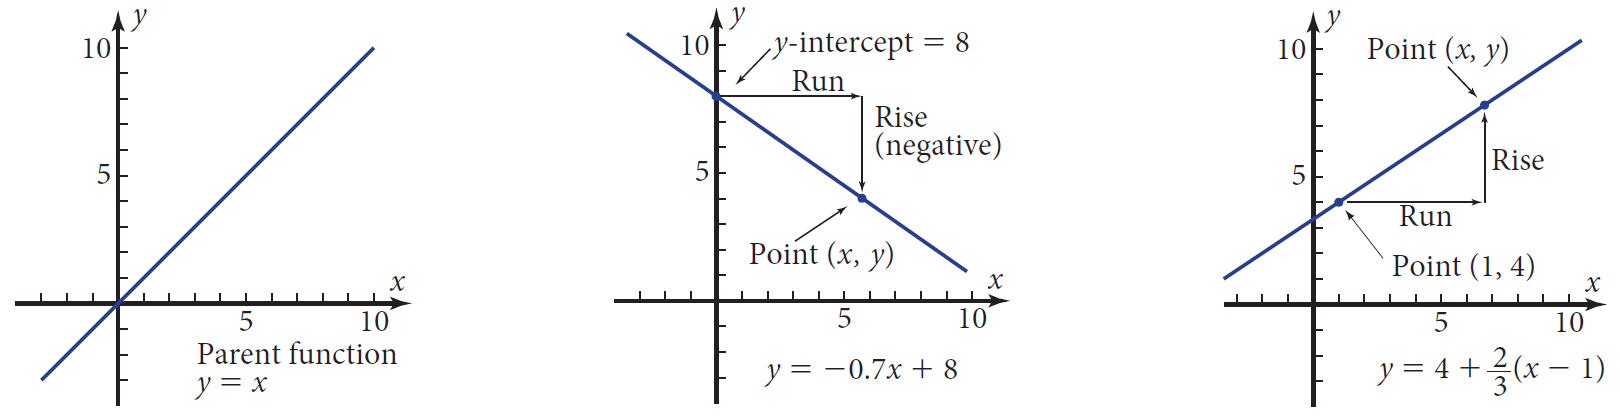
\includegraphics[width=1\textwidth]{figure/book1.png} % Adjust width here to scale the image
    \caption{Linear functions}
    \label{fig:book_image}
\end{figure}

The graph of a linear function is a straight line. The parent function \(y = x\) is shown on the left in figure \ref{fig:book_image}, the slope-intercept form in the middle, and the point-slope form on the right.

For the slope-intercept form: "Start at \(b\) on the \(y\)-axis, move \(x\) units horizontally, and rise \(ax\) units vertically." For the point-slope form: "Start at \((x_1, y_1)\), move \((x - x_1)\) units horizontally, and rise \(a(x - x_1)\) units vertically."

\subsection*{Quadratic Functions}
The general equation for a quadratic function is given by

\[
y = ax^2 + bx + c,
\]

where \(a \neq 0\), and \(a\), \(b\), and \(c\) are constants. The domain of this function is all real numbers.

\begin{figure}[h]
    \centering
    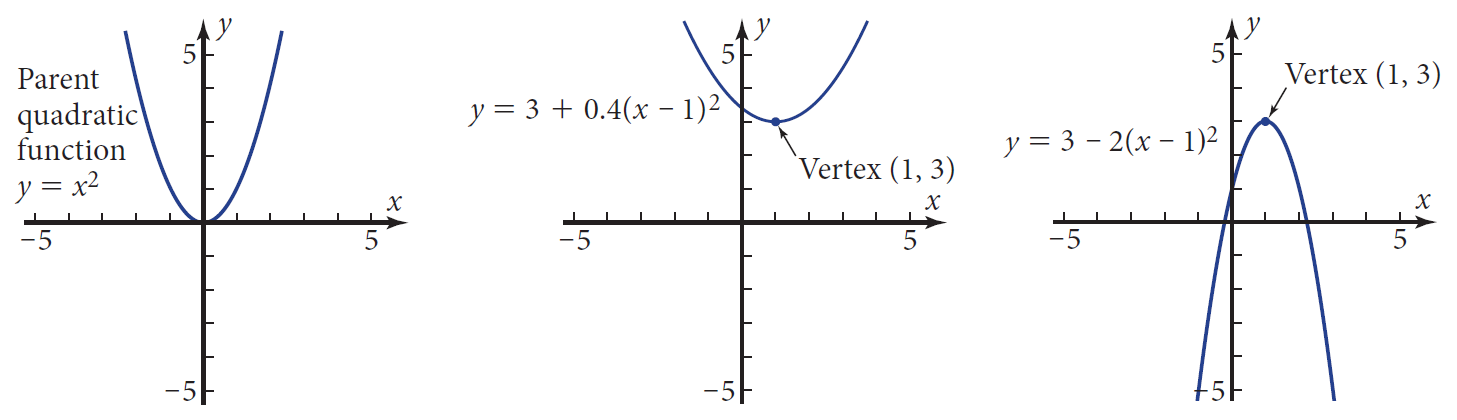
\includegraphics[width=1\textwidth]{figure/book2.png} % Adjust width here to scale the image
    \caption{Quadratic functions}
    \label{fig:book_image2}
\end{figure}

The parent function for a quadratic equation is

\[
y = x^2,
\]

where the vertex of the parabola is at the origin \((0, 0)\).

The transformed function can be written in vertex form as

\[
y = k + a(x-h)^2,
\]

where the vertex of the parabola is located at \((h, k)\). In this form:
\begin{itemize}
    \item \(k\) represents the vertical translation,
    \item \(h\) represents the horizontal translation,
    \item \(a\) represents the vertical dilation.
\end{itemize}

Vertex form can also be written as

\[
y - k = a(x-h)^2,
\]

but expressing \(y\) explicitly in terms of \(x\) makes the equation easier to enter into a graphing calculator.

The graph of a quadratic function is a parabola (from the Greek word for "along the path of a ball"). The parabola is concave up if \(a > 0\) and concave down if \(a < 0\). This behaviour is illustrated in figure \ref{fig:book_image2}.

\subsection*{Power Functions}
The general equation for a power function is given by

\[
y = ax^b,
\]

where \(a\) and \(b\) are nonzero constants. The domain of the function depends on the value of \(b\):
\begin{itemize}
    \item If \(b > 0\), the domain is all real numbers.
    \item If \(b < 0\), the domain excludes \(x = 0\) to avoid division by zero.
    \item If \(b\) is not an integer, the domain usually excludes negative numbers to avoid taking roots of negative numbers.
\end{itemize}
In most applications, the domain is restricted to non-negative numbers.

\begin{figure}[h]
    \centering
    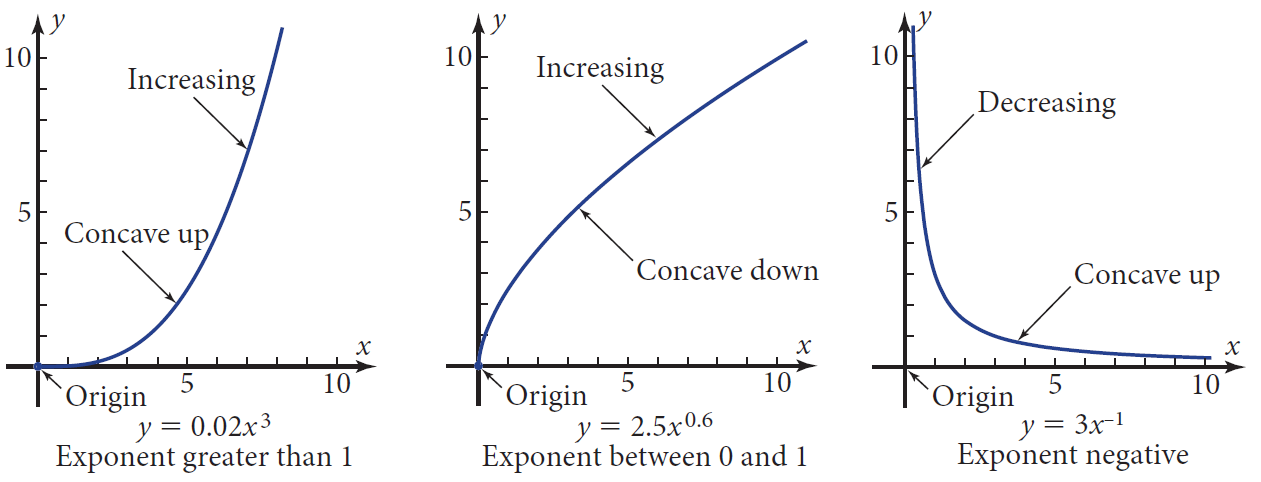
\includegraphics[width=1\textwidth]{figure/book3.png} % Adjust width here to scale the image
    \caption{Power functions}
    \label{fig:book_image3}
\end{figure}

The parent function for a power function is

\[
y = x^b.
\]

For the general power function \(y = ax^b\):
\begin{itemize}
    \item If \(b > 0\), then \(y\) varies directly with the \(b\)th power of \(x\), meaning \(y\) is directly proportional to the \(b\)th power of \(x\).
    \item If \(b < 0\), then \(y\) varies inversely with the \(b\)th power of \(x\), meaning \(y\) is inversely proportional to the \(b\)th power of \(x\).
\end{itemize}

The dilation factor \(a\) serves as the proportionality constant.

The translated form of a power function is

\[
y = d + a(x - c)^b,
\]

where \(c\) and \(d\) are the horizontal and vertical translations, respectively. This can be compared with the translated forms of linear and quadratic functions:

\[
\begin{aligned}
& y = y_1 + a(x - x_1) &\text{(linear function)}, \\
& y = k + a(x - h)^2 &\text{(quadratic function)}.
\end{aligned}
\]

Unless otherwise stated, "power function" will imply the untranslated form, \(y = ax^b\).

Figure \ref{fig:book_image3} shows the graphs of power functions for different values of \(b\). In all cases, \(a > 0\). The shape and concavity of the graph depend on the value of \(b\):
\begin{itemize}
    \item If \(b > 0\), the graph contains the origin.
    \item If \(b < 0\), the graph has the axes as asymptotes.
    \item The function is increasing if \(b > 0\) and decreasing if \(b < 0\).
    \item The graph is concave up if \(b > 1\) or \(b < 0\), and concave down if \(0 < b < 1\).
\end{itemize}
The concavity of the graph describes the rate at which \(y\) increases. For \(b > 0\), concave up indicates that \(y\) is increasing at an increasing rate, while concave down indicates that \(y\) is increasing at a decreasing rate.

\subsection*{Exponential Functions}

The general equation for an exponential function is given by

\[
y = a b^x,
\]

where \(a\) and \(b\) are constants, \(a \neq 0\), \(b > 0\), and \(b \neq 1\). The domain of this function is all real numbers.

The parent function for an exponential equation is

\[
y = b^x,
\]
where the asymptote is the \(x\)-axis.

\begin{figure}[h]
    \centering
    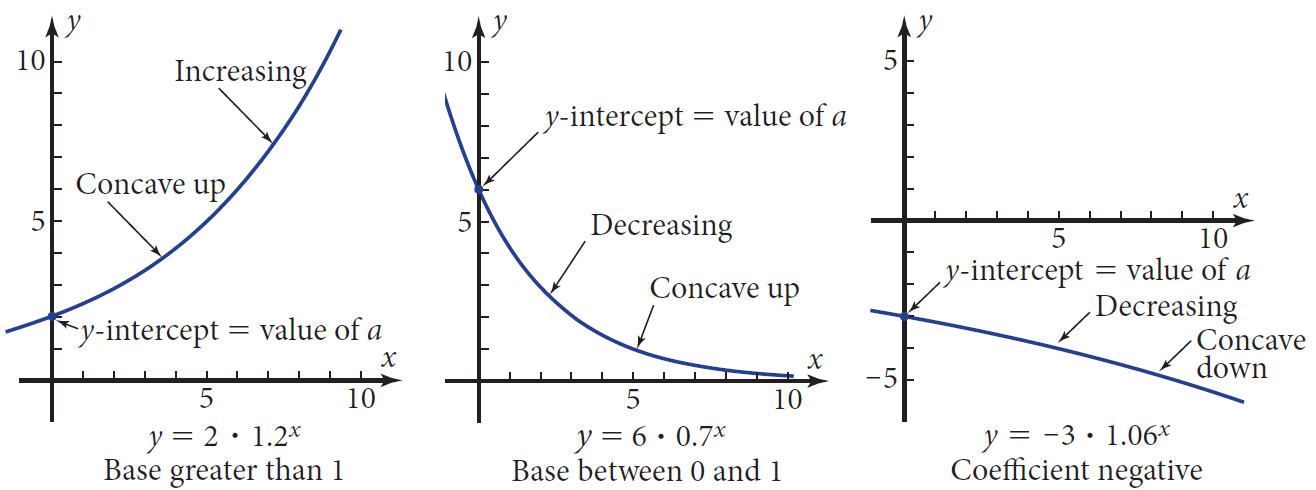
\includegraphics[width=1\textwidth]{figure/book4.png} % Adjust width here to scale the image
    \caption{Exponential functions}
    \label{fig:book_image4}
\end{figure}

In the equation \(y = a b^x\), we say that "\(y\) varies exponentially with \(x\)." This means that \(y\) changes by a constant factor \(b\) for each unit increase in \(x\).

The translated form of the exponential function is

\[
y = a b^x + c,
\]

where the asymptote is the line \(y = c\). Unless otherwise stated, "exponential function" will refer to the untranslated form \(y = a b^x\).

Figure \ref{fig:book_image4} illustrates exponential functions for different values of \(a\) and \(b\). The key properties of the graph are as follows:
\begin{itemize}
    \item The constant \(a\) is the \(y\)-intercept of the graph.
    \item The function is increasing if \(b > 1\) and decreasing if \(0 < b < 1\), provided \(a > 0\).
    \item If \(a < 0\), the function's behavior is reversed: it is decreasing if \(b > 1\) and increasing if \(0 < b < 1\).
    \item The graph is concave up if \(a > 0\) and concave down if \(a < 0\).
\end{itemize}

Mathematicians often use one of two particular constants as the base for an exponential function: either 10, which is the base of the decimal system, or the naturally occurring number \( e \), which approximately equals 2.71828. These bases are significant in various mathematical applications.

\begin{definition}{Special Exponential Functions}

\begin{align*}
y &= a \cdot 10^{bx} \hspace{1cm} \text{base-10 exponential function} \\
y &= a \cdot e^{bx}  \hspace{1.2cm} \text{natural (base-}e\text{) exponential function,}
\end{align*}

where $a$ and $b$ are constants and the domain is all real numbers.
    
\end{definition}

To generalise the exponential function, the variable in the exponent is often multiplied by a constant. The (untranslated) general forms of these exponential functions are given below:

\[
y = a \cdot 10^{bx}
\quad \text{and} \quad
y = a \cdot e^{bx}
\]

These functions can be further generalised by incorporating translations in both the \(x\)- and \(y\)-directions. The translated forms are:

\[
y = a \cdot 10^{b(x - c)} + d
\quad \text{and} \quad
y = a \cdot e^{b(x - c)} + d
\]

The base-\(e\) exponential function, in particular, has a significant advantage when studying calculus, as the rate of change of \(e^x\) is equal to \(e^x\) itself.

\section{Logarithms}
Any positive number can be written as a power of 10. For instance,

\[
\begin{aligned}
3 & = 10^{0.477 \ldots} \\
5 & = 10^{0.6989 \ldots} \\
15 & = 10^{1.1760 \ldots}
\end{aligned}
\]

The exponents \(0.4771 \ldots\), \(0.6989 \ldots\), and \(1.1760 \ldots\) are called the base-10 logarithms of 3, 5, and 15, respectively:

\[
\begin{aligned}
\log 3 & = 0.4771 \ldots \\
\log 5 & = 0.6989 \ldots \\
\log 15 & = 1.1760 \ldots
\end{aligned}
\]

To better understand the meaning of logarithms, press \texttt{LOG} 3 on your calculator. You will get:

\[
\log 3 = 0.477121254 \ldots
\]

Then, without rounding, raise 10 to this power. You will obtain:

\[
10^{0.477121254 \ldots} = 3
\]

The powers of 10 have the normal properties of exponentiation. For instance,
\[
\begin{aligned}
15 & = (3)(5) = \left(10^{0.4771 \ldots}\right)\left(10^{0.6999 \ldots}\right) \\
& = 10^{0.4771 \ldots + 0.6599 \ldots} \\
& = 10^{1.1760 \ldots}
\end{aligned}
\]

This means \(10^{0.4771 \ldots + 0.6599 \ldots} = 10^{1.1760 \ldots}\). Here, you add the exponents while keeping the same base. You can verify with your calculator that \(10^{1.1760 \ldots}\) indeed equals 15.

From this example, you can infer that logarithms have the same properties as exponents. This is expected because logarithms \textit{are} exponents. For instance,

\[
\log(3 \cdot 5) = \log 3 + \log 5 \quad \text{\textit{The logarithm of a product equals the sum of the logarithms of the factors}.}
\]

From the values given earlier, you can also show that:

\[
\log \frac{15}{3} = \log 15 - \log 3 \quad \text{\textit{The logarithm of a quotient}.}
\]

This property is reasonable because you divide powers of equal bases by subtracting the exponents:

\[
\frac{15}{3} = \frac{10^{1.1760 \ldots}}{10^{0.477 \ldots}} = 10^{1.1760 \ldots - 0.4771 \ldots} = 10^{0.6989 \ldots} = 5
\]

Since a power can be written as a product, you can find the logarithm of a power as follows:

\[
\begin{aligned}
\log 34 & = \log (3 \cdot 3 \cdot 3 \cdot 3) = \log 3 + \log 3 + \log 3 + \log 3 \\
& = 4 \log 3 \quad \text{\textit{Combine like terms}.}
\end{aligned}
\]

The logarithm of a power equals the exponent of that power times the logarithm of the base. To verify this result, observe that \(3^4 = 81\). Press \(4 \times \texttt{LOG}\,3\) on your calculator, and you'll find it equals \(1.9084 \ldots\).

\begin{definition}{Base-10 Logarithms}

\[
\log x=y \iff 10^y=x
\]

\textit{Verbally}: $\log x$ is the exponent in the power of 10 that gives $x$   
\end{definition}

The term logarithm comes from the Greek words \emph{logos}, meaning "ratio," and \emph{arithmos}, meaning "number." Before the invention of calculators, base-10 logarithms were calculated approximately using infinite series and recorded in tables. Products involving many factors, such as
\[
(357)(4.367)(22.4)(3.142)
\]
could be calculated by adding their logarithms (exponents) rather than tediously multiplying several pairs of numbers. This method was invented by Englishman Henry Briggs (1561–1630) and Scotsman John Napier (1550–1616). The name logarithm, thus, reflects this "logical way to do arithmetic".

\begin{custombox}{Properties of base-10 logarithms}
\begin{itemize}
    \item Log of a Product:
    
    \[
    \log x y=\log x+\log y
    \]
    
    \textit{Verbally}: The $\log$ of a product equals the sum of the logs of the factors.
    \vspace{0.2cm}
    \item Log of a Quotient:
    
    \[
    \log \frac{x}{y}=\log x-\log y
    \]
    \vspace{0.1cm}
    \textit{Verbally}: The $\log$ of a quotient equals the log of the numerator minus the $\log$ of the denominator.
    \vspace{0.2cm}
    \item Log of a Power:
    \[
    \log x^y=y \log x
    \]
    \textit{Verbally}: The $\log$ of a power equals the exponent times the log of the base.
\end{itemize}

   
\end{custombox}

\begin{example} Find $x$ if $\log_{10} 10^{3.721}=x$

\begin{solution}
By definition, the logarithm is the exponent of 10. So $x=3.721$.
\end{solution}
\end{example}

\begin{example} Find $x$ if $0.258=10^x$

\begin{solution}
   By definition, $x$, the exponent of 10 , is the logarithm of 0.258 .

    \[
    x=\log_{10} 0.258=-0.5883 \ldots
    \]
\end{solution}
    
\end{example}

\begin{custombox}{The most important thing to remember about logarithms is this}
    \textbf{A logarithm is an exponent.}
\end{custombox}

\subsection*{Logarithms with Any Base: The Change-of-Base Property}
If \(x = 10^y\), then \(y\) is the base-10 logarithm of \(x\). Similarly, if \(x = 2^y\), then \(y\) is the base-2 logarithm of \(x\). The only difference between these logarithms is the number that serves as the base. To distinguish among logarithms with different bases, the base is written as a subscript after the abbreviation "log." For instance:

\[
\begin{aligned}
3 &= \log_2 8 \Leftrightarrow 2^3 = 8, \\
4 &= \log_3 81 \Leftrightarrow 3^4 = 81, \\
2 &= \log_{10} 100 \Leftrightarrow 10^2 = 100.
\end{aligned}
\]

The symbol \(\log_2 8\) is pronounced "log to the base 2 of 8." The symbol \(\log_{10} 100\) is, of course, equivalent to \(\log 100\), as defined in the previous section. Note that in all cases, a logarithm represents an exponent.

\begin{definition}{Logarithm with Any Base}
\textit{Algebraically}:

\hspace{1cm}$\log _b x=y$ if and only if $b^y=x, \quad$ where $b>0, b \neq 1$, and $x>0$

\vspace{0.3cm}

\textit{Verbally}:

\hspace{1cm} $\log _b x=y$ means that $y$ is the exponent of $b$ that gives $x$ as the answer.
    
\end{definition}

The way you pronounce the symbol for logarithm gives you a way to remember the definition. The next two examples show you how to do this.

\begin{example} Write $\log _5 c=a$ in exponential form.

\begin{solution}

Think this:
\begin{itemize}
    \item "\(\log_5 \ldots\)" is read as "log base 5 \(\ldots\)," meaning 5 is the base.
    \item A logarithm is an exponent. Since the \(\log\) equals \(a\), \(a\) must be the exponent.
    \item The "answer" obtained from \(5^a\) is the argument of the logarithm, denoted as \(c\).
\end{itemize}

Write only this: 

\[
5^a = c
\]
\end{solution}
\end{example}

\begin{example} Write $z^4=m$ in logarithmic form.

\begin{solution}
    $\log _z m=4$
\end{solution}
    
\end{example}

Two bases of logarithms are used frequently enough to have their own key on most calculators. One is the base-10 logarithm, also known as the common logarithm, as discussed in the previous section. The other is the base-\(e\) logarithm, known as the natural logarithm, where \(e = 2.71828 \ldots\), a naturally occurring number (like \(\pi\)) that will be advantageous in your future mathematical studies.

The symbol \(\ln x\) (pronounced "el en of \(x\)") is used for natural logarithms, and is defined as:
\[
\ln x = \log_e x
\]

\begin{definition}{Common Logarithm and Natural Logarithm}
\hspace{1cm} \textit{Common}: The symbol $\log x$ means $\log _{10} x$.

\hspace{1cm}  \textit{Natural}: \hspace{0.2cm}The symbol $\ln x$ means $\log _e x$, where $e$ is a constant equal to $2.71828182845 \ldots$
\end{definition}

\begin{example} Find $\log _5 17$. Check your answer by an appropriate numerical method.

\begin{solution} Let $x=\log _5 17$.

\begin{equation*}
\begin{aligned}
& 5^x=17 \\
& \log _{10} 5^x=\log _{10} 17 \\
& x \log _{10} 5=\log _{10} 17 \\
& x=\frac{\log _{10} 17}{\log _{10} 5}=1.7603 \ldots \\
& \log _5 17=1.7603 \ldots \\
& 5^{1.7603 \ldots}=17
\end{aligned}
\end{equation*}
\end{solution}
\end{example}

In this example, note that the base-5 logarithm of a number is directly proportional to the base-10 logarithm of that number. The conclusion of the example can be expressed as follows:

\[
\log_5 17 = \frac{1}{\log_{10} 5} \cdot \log_{10} 17 = 1.4306 \ldots \log_{10} 17
\]

To find the base-5 logarithm of any number, simply multiply its base-10 logarithm by \(1.4306 \ldots\) (that is, divide by \(\log_{10} 5\)).

This proportional relationship is known as the change-of-base property. From the results of Example 3, you can write:

\[
\log_5 17 = \frac{\log_{10} 17}{\log_{10} 5}
\]

Notice that the logarithm with the desired base is isolated on the left side of the equation, while the two logarithms on the right side share the same base—typically one that is available on your calculator. The box below illustrates this property for bases \(a\) and \(b\) with argument \(x\):

\begin{custombox}{The Change-of-Base Property of Logarithms}

\begin{equation*}
\log _a x=\frac{\log _b x}{\log _b a} \quad \text { or } \quad \log _a x=\frac{1}{\log _b a}\left(\log _b x\right)
\end{equation*}
    
\end{custombox}

\begin{example}
Find $\ln 29$ using the change-of-base property with base-10 logarithms. Check your answer directly by pressing $\ln 29$ on your calculator.

\begin{solution}

\[
\ln 29=\frac{\log 29}{\log e}=\frac{1.4623 \ldots}{0.4342 \ldots}=3.3672 \ldots
\]

\hspace{0.9cm} Directly: $\quad \ln 29=3.3672 \ldots,$

which agrees with the answer we got using the change-of-base property.
\end{solution}
\end{example}

\begin{custombox}{Properties of Logarithms}
\setlength{\leftskip}{1cm}  % Reset the text indent
\setlength{\rightskip}{1cm} % Reset the right indent
The Logarithm of a Power:
$$
\log _b x^y=y \log _b x
$$

\textit{Verbally}: The logarithm of a power equals the product of the exponent and the logarithm of the base.
\vspace{0.5cm}
The Logarithm of a Product:
$$
\log _b(x y)=\log _b x+\log _b y
$$
\textit{Verbally}: The logarithm of a product equals the sum of the logarithms of the factors.
\vspace{0.5cm}
The Logarithm of a Quotient:
$$
\log _b \frac{x}{y}=\log _b x-\log _b y
$$

\textit{Verbally}: The logarithm of a quotient equals the logarithm of the numerator minus the logarithm of the denominator.

\setlength{\leftskip}{0cm}  % Reset the text indent
\setlength{\rightskip}{0cm} % Reset the right indent

\end{custombox}

\subsection*{Solving Exponential and Logarithmic Equations}
Logarithms provide a way to solve an equation with a variable in the exponent or to solve an equation that already contains logarithms. We will demonstrate this through the next few examples.

\begin{example} Solve the exponential equation $7^{3 x}=983$ algebraically, using logarithms.

\begin{solution}
\begin{align*}
& 7^{3x} = 983  \\
& \log 7^{3x} = \log 983 && \texttt{\small Take the base-10 logarithm of both sides.} \\
& 3x \log 7 = \log 983 && \texttt{\small Apply the logarithm power property.} \\
& x = \frac{\log 983}{3 \log 7} && \texttt{\small Divide both sides by the coefficient of x.}\\
& x = 1.1803 \ldots   
\end{align*}


\end{solution}
    
\end{example}

\begin{example} Solve the equation
    \begin{equation*}
\log _2(x-1)+\log _2(x-3)=3
\end{equation*}

\begin{solution}

\begin{align*}
& \log _2(x-1)+\log _2(x-3)=3  \\
& \log _2[(x-1)(x-3)]=3 && \texttt{\small Apply the logarithm of a product property.} \\
& 2^3=(x-1)(x-3) && \texttt{\small Use the definition of logarithm.} \\
& 8=x^2-4 x+3 && \texttt{\small Expand the product.}\\
& x^2-4 x-5=0 && \texttt{\small Reduce one side to zero. Use the symmetric }\\
&\vspace{-0.2cm}   && \texttt{\small property of equality.} \\
& (x-5)(x+1)=0 && \texttt{\small Solve by factoring.} \\
& x=5 \quad \text{ or } \quad x=-1
\end{align*}
We need to be cautious here because the solutions in the final step are the solutions of the quadratic equation, and we must make sure they are also solutions of the original logarithmic equation. Check by substituting the solutions into the original equation.

\begin{minipage}[t]{0.45\textwidth}
If $x=5$, then
\[
\begin{aligned}
& \log _2(5-1)+\log _2(5-3) \\
& =\log _2 4+\log _2 2 \\
& =2+1=3
\end{aligned}
\]
\end{minipage}%
\hfill
\begin{minipage}[t]{0.45\textwidth}
If $x=-1$, then
\[
\begin{aligned}
& \log _2(-1-1)+\log _2(-1-3) \\
& =\log _2(-2)+\log _2(-4)
\end{aligned}
\]
which is undefined.
\end{minipage}

\end{solution}

\end{example}

\begin{example} Solve the equation

\[
e^{2 x}-3 e^x+2=0
\]

\begin{solution}

\[
\begin{aligned}
& e^{2 x}-3 e^x+2=0 \\
& \left(e^x\right)^2-3 e^x+2=0
\end{aligned}
\]
We realise that this is a quadratic equation in the variable $e^x$. Using the quadratic formula, you get

\[
\begin{aligned}
& e^x=\frac{+3 \pm \sqrt{9-4(2)}}{2}=\frac{3 \pm 1}{2} \\
& e^x=2 \text { or } e^x=1
\end{aligned}
\]


You now have to solve these two equations.
\[
\begin{array}{ll}
e^x=2 & \qquad e^x=1 \\
x=\ln 2=0.6931 \ldots & \qquad x=0
\end{array}
\]
Check:

\[
\begin{array}{ll}
e^{2 \ln 2}-3 e^{\ln 2}+2 & \qquad \left(e^0\right)^2-3 e^0+2 \\
=\left(e^{\ln 2}\right)^2-3 e^{\ln 2}+2 & \qquad =1^2-3(1)+2=0 \\
=2^2-3(2)+2=0 &
\end{array}
\]
Both solutions are correct.
\end{solution}  
\end{example}

\begin{example} Solve the logarithmic equation $\ln (x+3)+\ln (x+5)=0$

\begin{solution}
    \[
\begin{aligned}
& \ln (x+3)+\ln (x+5)=0 \\
& \ln [(x+3)(x+5)]=0 \\
& (x+3)(x+5)=e^0=1 \\
& x^2+8 x+15=1 \\
& x^2+8 x+14=0 \\
& x=-2.5857 \ldots \quad \text { or } \qquad x=-5.4142 \ldots
\end{aligned}
\]
Check:
\[
\begin{aligned}
& x=-2.5857 \ldots: \\
& \ln (-2.5857 \ldots+3)+\ln (-2.5857 \ldots+5) \\
& =\ln (0.4142 \ldots)+\ln (2.4142 \ldots) \\
& =-0.8813 \ldots+0.8813 \ldots=0
\end{aligned}
\]
which is ok.

\[
\begin{aligned}
& x=-5.4142 \ldots: \\
& \ln (-5.4142 \ldots+3)+\ln (-5.4142 \ldots+5) \\
& =\ln (-2.4142 \ldots)+\ln (-0.4142 \ldots)
\end{aligned}
\]

which is undefined.

The only valid solution is $x=-2.5857 \ldots$.
\end{solution}
    
\end{example}

